\chapter{Tests and Results}

\section{Introduction}
After presenting the design and implementation of the various modules that make up our system, we now move on to the testing and evaluation phase. This chapter places particular emphasis on assessing the wheat disease classification approach, as it represents the core component and the primary objective of our system. Through a series of carefully designed experiments, we aim to evaluate the effectiveness and performance of the proposed hierarchical classification strategy.

We begin by outlining the evaluation metrics employed, followed by a presentation of the experiment objectives. The results are then detailed and analyzed, with a specific focus on the performance of the disease classification models. Lastly, we compare our findings with existing state-of-the-art methods to highlight the strengths and contributions of our approach.



\section{Evaluation Metrics}

We used several widely recognized evaluation metrics to assess our classification models' performance. These metrics help quantify the models' effectiveness in correctly identifying and classifying wheat diseases and insect pests.

A confusion matrix is a tabular representation of the actual versus predicted classifications. It provides a comprehensive view of model performance across all classes, showing true positives (TP), true negatives (TN), false positives (FP), and false negatives (FN) for each class.

\begin{itemize}
    \item \textbf{Accuracy:} Measures the proportion of correct predictions (both true positives and true negatives) among the total number of predictions, as shown in Equation~\ref{eq:accuracy}.
    \begin{equation}
        \text{Accuracy} = \frac{TP + TN}{TP + TN + FP + FN}
        \label{eq:accuracy}
    \end{equation}

    \item \textbf{Precision:} Indicates the proportion of correctly predicted positive observations to the total predicted positives. It is useful when the cost of false positives is high (Equation~\ref{eq:precision}).
    \begin{equation}
        \text{Precision} = \frac{TP}{TP + FP}
        \label{eq:precision}
    \end{equation}

    \item \textbf{Recall:} Measures the proportion of correctly predicted positive observations out of all actual positives. It is important when the cost of false negatives is high (Equation~\ref{eq:recall}).
    \begin{equation}
        \text{Recall} = \frac{TP}{TP + FN}
        \label{eq:recall}
    \end{equation}

    \item \textbf{F1-score:} The harmonic mean of precision and recall. It balances the two, especially when the class distribution is uneven (Equation~\ref{eq:f1score}).
    \begin{equation}
        \text{F1-score} = 2 \cdot \frac{\text{Precision} \cdot \text{Recall}}{\text{Precision} + \text{Recall}}
        \label{eq:f1score}
    \end{equation}
\end{itemize}

For the insect pest detection task, we also considered additional metrics widely used in object detection tasks:

\begin{itemize}
    \item \textbf{Mean Average Precision at IoU 0.5 (mAP@0.5):} Evaluates the model’s ability to detect pests correctly at an Intersection over Union (IoU) threshold of 0.5. It calculates the average precision across all classes and provides an overall measure of detection accuracy.

    \item \textbf{Mean Precision:} Represents the average of precision values across all insect pest classes.

    \item \textbf{Mean Recall:} Represents the average of recall values across all insect pest classes.
\end{itemize}

These metrics provide a holistic evaluation of the model's ability to classify and detect both wheat diseases and insect pests effectively in real-world conditions.



\section{Objectives of the experiments}
The main objective of our experiments is to justify the choices made during the design and implementation of our system. This includes evaluating the different CNN architectures used, as well as the selection of optimizers and technologies such as attention mechanisms. Each component was chosen based on its potential to enhance the model’s performance in detecting and classifying wheat diseases.

Moreover, we aim to improve the effectiveness of the hierarchical classification approach, which is central to our system. By conducting various tests and comparisons, we seek to assess how this approach performs under different configurations and against alternative strategies.

Finally, we intend to evaluate the robustness of our dataset by applying it to models proposed in related studies. This comparison will help us understand how well our data generalizes and how it supports model performance in broader applications.


\section{Experimental results in wheat disease classification models}

We defined two distinct test scenarios to evaluate our system. The first scenario focuses on testing the binary classification model, which is designed to classify whether a given sample is healthy or diseased. The second scenario evaluates the multiclass classification mode to identify the specific disease category affecting the sample.

\subsection{Scenario 1: Testing of binary classification model}
In this scenario, we will investigate the performance of multiple CNN architectures as feature extractors and assess their integration with a range of traditional machine learning classifiers to determine the most effective combinations for our task.
\subsubsection{Testing different CNN architectures for feature extraction}
This section explores the effectiveness of various pretrained convolutional neural network (CNN) architectures for image feature extraction. By evaluating the quality of extracted features using unsupervised clustering metrics, the goal is to identify models that best capture discriminative patterns while balancing accuracy, dimensionality, and computational cost.

\paragraph{Load and preprocess the dataset:}  
The dataset $D_1$ is prepared by normalizing image pixel values to a $[0, 1]$ scale, selecting 80\% of the data for training, and loading this subset in a fixed order to maintain the correct association between images and their labels during feature extraction.

\paragraph{Define pretrained CNN architectures:}  
A set of pretrained CNN architectures, such as \textit{EfficientNetB2}, \textit{MobileNet}, \textit{VGG19}, \textit{Xception}, \textit{InceptionV3}, \textit{DenseNet169}, \textit{DenseNet201}, \textit{ResNet50V2}, and \textit{ResNet101V2}, all trained on the ImageNet dataset, are used as feature extractors. These models are applied without their original classification layers and fixed during evaluation to ensure they only generate feature representations. The model outputs a one-dimensional feature vector for each input image using global average pooling, capturing the most relevant high-level information from the image.

\paragraph{Extract features and evaluate feature quality using clustering metrics:}  
Deep features are extracted from each image in the training set using the selected CNN architectures. The resulting feature vectors, along with their corresponding class labels, are collected for further analysis.

To evaluate the discriminative power of these features without relying on a supervised classifier, two unsupervised clustering metrics are employed:

\begin{itemize}
    \item \textbf{Silhouette Score}:  
    The Silhouette Score combines cohesion (how close a point is to others in the same class) and separation (how far it is from points in other classes). For a single sample $i$, the silhouette coefficient is calculated as shown in Equation~\ref{eq:silhouette}:
    \begin{equation}
        s(i) = \frac{b(i) - a(i)}{\max(a(i), b(i))}
        \label{eq:silhouette}
    \end{equation}
    where $a(i)$ is the average distance to other points in the same class, and $b(i)$ is the minimum average distance to points in a different class. The score ranges from $-1$ to $1$, with values closer to $1$ indicating well-clustered data.

    \item \textbf{Davies–Bouldin Score (DBI)}:  
    The Davies–Bouldin Score evaluates intra-cluster similarity relative to inter-cluster differences. It is calculated as shown in Equation~\ref{eq:dbi}:
    \begin{equation}
        \text{DBI} = \frac{1}{n} \sum_{i=1}^{n} \max_{j \neq i} \left( \frac{\sigma_i + \sigma_j}{d_{ij}} \right)
        \label{eq:dbi}
    \end{equation}
    where $\sigma_i$ is the average distance between each point in cluster $i$ and the centroid of that cluster, and $d_{ij}$ is the distance between the centroids of clusters $i$ and $j$. Lower DBI values indicate better separation and more compact clusters.
\end{itemize}


\paragraph{Compare and summarize results:}  
Figure~\ref{fig:cnn-results} presents the results of applying various pre-trained CNN architectures for feature extraction. Based on the comparison, the three best-performing models are \textbf{EfficientNetB2}, \textbf{VGG19}, and \textbf{DenseNet169}.

\begin{itemize}
    \item \textbf{EfficientNetB2} achieved the highest silhouette score (0.034) and a reasonable extraction time (38.14 s) with moderate feature dimensionality (1408), making it a strong candidate for capturing discriminative features while maintaining computational efficiency.

    \item \textbf{VGG19}, despite its longer processing time (112.41 s), produced the lowest DB score (6.368) and the smallest feature dimension (512), indicating highly compact and well-separated feature representations suitable for clustering.

    \item \textbf{DenseNet169} also showed competitive clustering performance with a silhouette score of 0.020, a DB score of 6.739, an acceptable dimensionality (1664), and moderate time cost (53.28 s), offering a good balance between quality and efficiency.
\end{itemize}

These models were selected for their ability to extract informative and discriminative features while maintaining trade-offs between accuracy, compactness, and processing time.


\begin{figure}[H] % 'H' needs \usepackage{float}
    \centering
    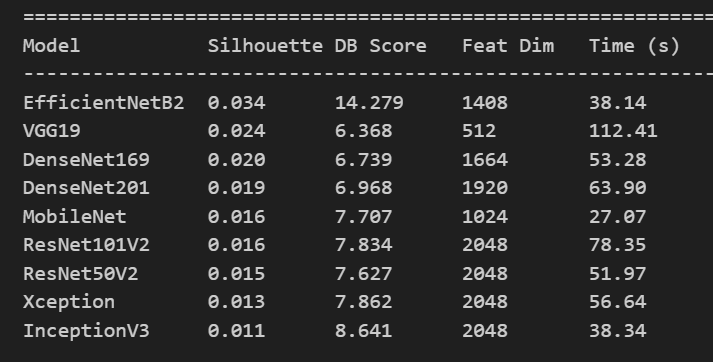
\includegraphics[width=0.9\textwidth]{chapters/chapter6/images/Figure01.png}
    \caption{ Performance comparison of pre-trained CNN architectures for feature extraction based on clustering metrics, feature dimensionality, and extraction time.}
    \label{fig:cnn-results}
\end{figure}


\subsubsection{Testing different machine learning models for classification}

In this experiment, EfficientNetB2, VGG19, and DenseNet169 were selected as the feature extractors, based on their strong performance in the previous evaluation. To enhance the model’s generalization and robustness, the D1 dataset was augmented using a combination of techniques, including gamma correction, CutOut, Mixup, and CutMix. Features extracted from each CNN were then used to train and evaluate multiple machine learning classifiers for binary classification: Decision Tree (DT), Random Forest (RF), Support Vector Machine (SVM), and Multi-Layer Perceptron (MLP). A comprehensive grid search was performed to optimize the hyperparameters of each classifier (as detailed in Table~\ref{tab:hyperparams}). The models were assessed using standard classification metrics, including accuracy, recall, precision, and F1-score (see Table~\ref{tab:performance}). Among the evaluated classifiers, the SVM achieved the best overall performance, demonstrating its effectiveness in leveraging the extracted features for accurate classification.

\begin{table}[h]
    \centering
    \renewcommand{\arraystretch}{1.5}
    \setlength{\tabcolsep}{8pt}
    \caption{\textit{Classifier hyperparameter grid search.}}
    \label{tab:hyperparams}
    \begin{tabular}{|p{1.5cm}|p{5.2cm}|p{5.3cm}|}
        \hline
        \textbf{Classifier} & \textbf{Hyperparameter} & \textbf{Explored Values} \\ \hline

        \multirow{4}{*}{SVM} 
        & Regularization parameter ($C$) & \{0.1, 1, 10\} \\ \cline{2-3}
        & Kernel type & \{linear, rbf, poly\} \\ \cline{2-3}
        & Kernel coefficient ($\gamma$) & \{scale, auto\} \\ \cline{2-3}
        & Polynomial degree (for poly kernel) & \{2, 3, 4\} \\ \hline

        \multirow{4}{*}{MLP} 
        & Hidden layer sizes & (50), (100), (100, 50) \\ \cline{2-3}
        & Activation function & \{ReLU, tanh\} \\ \cline{2-3}
        & Optimizer & \{adam, sgd\} \\ \cline{2-3}
        & Learning rate strategy & \{constant, adaptive\} \\ \hline

        \multirow{4}{*}{RF} 
        & Number of estimators & \{50, 100, 200\} \\ \cline{2-3}
        & Max features & \{sqrt, log2\} \\ \cline{2-3}
        & Min samples per leaf & \{1, 2, 5\} \\ \cline{2-3}
        & Min samples to split & \{2, 5, 10\} \\ \hline

        \multirow{3}{*}{DT} 
        & Maximum depth & \{50, 100, 200\} \\ \cline{2-3}
        & Split criterion & \{gini, entropy\} \\ \cline{2-3}
        & Min samples per leaf & \{1, 2, 5\} \\ \hline
    \end{tabular}
\end{table}



\vspace{1cm}

\begin{table}[h]
    \centering
    \renewcommand{\arraystretch}{1.4}
    \setlength{\tabcolsep}{10pt}
    \caption{Performance of machine learning classifiers using CNN feature extraction on the augmented D1 dataset.}
    \label{tab:performance}
    \begin{tabular}{|p{2.5cm}|p{4cm}|c|c|c|c|}
        \hline
        \textbf{Dataset} & \textbf{Classifier} & \textbf{Accuracy} & \textbf{Recall} & \textbf{Precision} & \textbf{F1-Score} \\ \hline
        
        \multirow{4}{*}{Augmented D1} 
        & Random Forest (RF) & 0.9867 & 0.9852 & 0.9880 & 0.9865 \\ \cline{2-6}
        & Decision Tree (DT) & 0.9547 & 0.9553 & 0.9534 & 0.9543 \\ \cline{2-6}
        & Support Vector Machine (SVM) & \textbf{0.9960} & \textbf{0.9958} & \textbf{0.9961} & \textbf{0.9960} \\ \cline{2-6}
        & Multilayer Perceptron (MLP) & 0.9940 & 0.9940 & 0.9939 & 0.9939 \\ \hline
    \end{tabular}
\end{table}





\subsection{Scenario 2: Testing of multiclass disease classification model}
This scenario involves testing \gls{abb:cnn} architectures with optimizers (\gls{abb:adam}, \gls{abb:sgd}) for feature extraction and examining the effect of different attention mechanisms on multiclass disease classification.

\subsubsection{Testing different CNN architectures with optimizers for feature extraction}
In this experiment, we systematically evaluated the influence of various convolutional neural network (CNN) architectures combined with different optimization algorithms on the performance of multiclass classification tasks. We utilized CNNs not only for feature extraction but also for the end-to-end classification process, allowing the networks to learn both robust feature representations and decision boundaries simultaneously. The dataset employed, referred to as D2, incorporated extensive data augmentation techniques as described in Section~\ref{sec:data_augmentation} , which helped improve model generalization by increasing the diversity of the training samples.

For each CNN architecture, we tested two widely used optimizers, Stochastic Gradient Descent (SGD) and Adaptive Moment Estimation (ADAM), to analyze how the choice of optimization strategy affects the training dynamics and final model accuracy. Model performance was rigorously evaluated using four key metrics: accuracy, recall, precision, and F1-score, providing a comprehensive understanding of classification effectiveness from multiple perspectives, including overall correctness, sensitivity to positive classes, and balance between precision and recall.

\begin{table}[h]
    \centering
    \renewcommand{\arraystretch}{1.4}
    \setlength{\tabcolsep}{10pt}
    \caption{Classification performance of CNN architectures using SGD and Adam optimizers.}
    \label{tab:cnn_performance}
    \begin{tabular}{|p{4cm}|p{2cm}|c|c|c|c|}
        \hline
        \textbf{CNN Architecture} & \textbf{Optimizer} & \textbf{Accuracy} & \textbf{Recall} & \textbf{Precision} & \textbf{F1-Score} \\ \hline

        \multirow{2}{*}{EfficientNetB2} 
        & SGD  & 96.57\% & 95.54\% & 94.34\% & 94.73\% \\ \cline{2-6}
        & Adam & 98.10\% & 96.94\% & 97.51\% & 97.22\% \\ \hline

        \multirow{2}{*}{MobileNet} 
        & SGD  & 94.29\% & 90.87\% & 94.14\% & 91.97\% \\ \cline{2-6}
        & Adam & 95.81\% & 94.02\% & 94.98\% & 94.45\% \\ \hline

        \multirow{2}{*}{Xception} 
        & SGD  & 96.99\% & 96.16\% & 96.40\% & 96.25\% \\ \cline{2-6}
        & Adam & 96.61\% & 94.11\% & 95.77\% & 94.86\% \\ \hline

        \multirow{2}{*}{InceptionV3} 
        & SGD  & 97.90\% & 97.47\% & 98.19\% & 97.81\% \\ \cline{2-6}
        & Adam & 92.38\% & 93.43\% & 89.91\% & 91.05\% \\ \hline

        \multirow{2}{*}{DenseNet201} 
        & SGD  & 98.87\% & 97.99\% & 98.43\% & 98.19\% \\ \cline{2-6}
        & Adam & 95.86\% & 94.87\% & 95.13\% & 94.97\% \\ \hline

        \multirow{2}{*}{ResNet50V2} 
        & SGD  & \textbf{99.25\%} & \textbf{99.35\%} & \textbf{98.80\%} & \textbf{99.04\%} \\ \cline{2-6}
        & Adam & 92.28\% & 89.67\% & 92.27\% & 90.57\% \\ \hline
    \end{tabular}
\end{table}

\vspace{0.5cm}

As summarized in Table~\ref{tab:cnn_performance}, the ResNet50V2 architecture coupled with the SGD optimizer consistently delivered superior results, achieving an accuracy of 99.25\%, a recall of 99.35\%, a precision of 98.80\%, and an F1-score of 99.04\%. These results indicate that this combination is highly effective at extracting discriminative features that enable the model to distinguish between classes with remarkable precision and reliability.



\subsubsection{Testing different attention mechanisms}
This experiment investigates the effectiveness of different attention mechanisms integrated into CNN architectures for improving multiclass classification performance. Attention modules such as Self-Attention, Squeeze-and-Excitation (SE), Convolutional Block Attention Module (CBAM), and Efficient Channel Attention (ECA) are evaluated using the dataset D2. These mechanisms aim to enhance feature representation by allowing the model to focus on the most informative parts of the input. The details and functioning principles of Self-attention, SE, and CBAM are explained in Appendix \ref{app:annexA}.


\begin{table}[h!]
\centering
\caption{Performance comparison of attention mechanisms.}
\label{tab:attention_mechanisms}
\begin{tabular}{|c|c|c|c|c|}
\hline
\textbf{Attention Mechanism} & \textbf{Test Accuracy} & \textbf{Recall} & \textbf{Precision} & \textbf{F1 Score} \\
\hline
Self-Attention              & 99.83\% & 99.77\% & 99.78\% & 99.79\% \\
\hline
SE (Squeeze-and-Excitation)& 99.81\% & 99.76\% & 99.77\% & 99.79\% \\
\hline
CBAM                       & 99.75\% & 99.69\% & 99.68\% & 99.70\% \\
\hline
ECA                        & 99.83\% & 99.78\% & 99.79\% & 99.81\% \\
\hline
\end{tabular}
\end{table}

\vspace{0.5cm}

On the augmented D2 dataset, the model incorporating the Efficient Channel Attention (ECA) mechanism delivered the best overall performance across all evaluation metrics, as shown in Table~\ref{tab:attention_mechanisms}, demonstrating its ability to enhance feature representations and improve classification accuracy effectively. Not far behind, the model integrated with the Self-Attention mechanism achieved similarly strong and balanced results, reflecting its capacity to capture long-range dependencies between features. 

This is further illustrated in Figure~\ref{fig:confusion_matrix}, which presents the confusion matrix for the ResNet50 model enhanced with the ECA attention mechanism, highlighting its strong ability to distinguish between classes with minimal misclassifications.

\begin{figure}[h!]
\centering
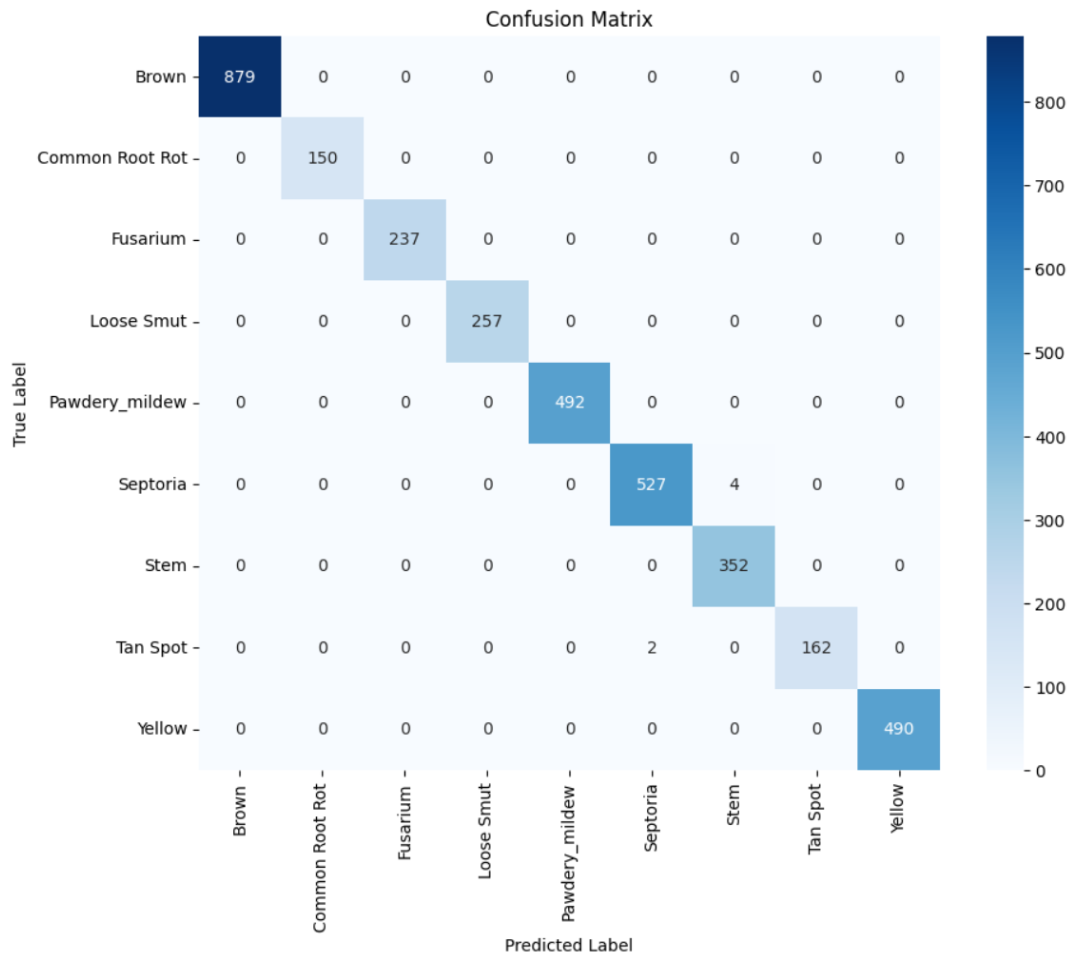
\includegraphics[width=0.7\textwidth]{chapters/chapter6/images/Figure02.png}
\caption{Confusion matrix of the multiclass classification model (ResNet50 + ECA attention mechanism).}
\label{fig:confusion_matrix}
\end{figure}


\textbf{Grad-CAM visualization} \\

To gain deeper insight into how different attention mechanisms influence the model’s decision-making process, we employed Grad-CAM (Gradient-weighted Class Activation Mapping). This technique provides visual explanations by highlighting the most relevant regions of the input image that contribute to the final prediction.

\begin{figure}[h!]
\centering
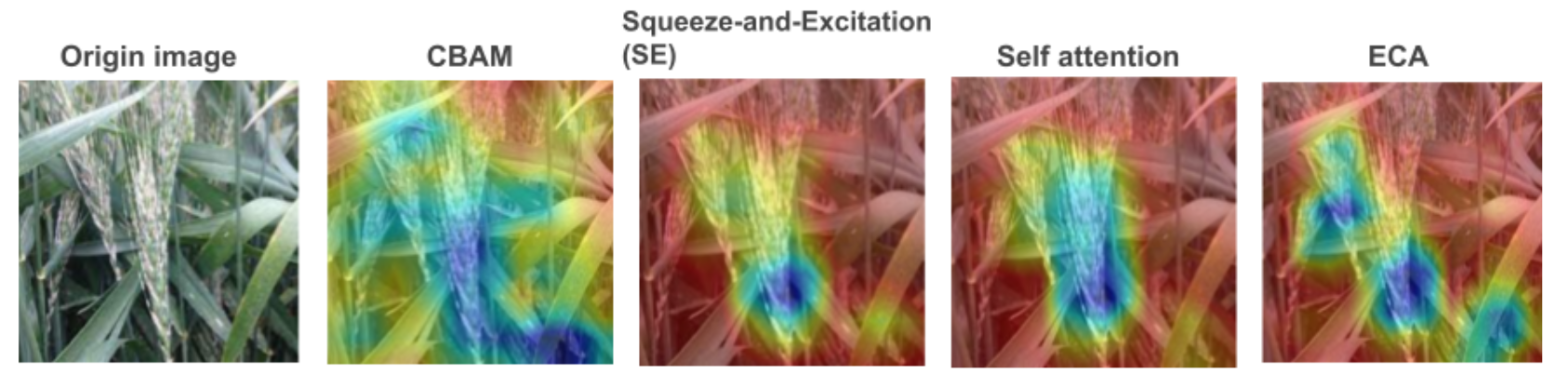
\includegraphics[width=0.9\textwidth]{chapters/chapter6/images/Figure03.png}
\caption{Grad-CAM Visualization of Different Attention Mechanisms: SE, CBAM, ECA, and Self-Attention.}
\label{fig:grad_cam}
\end{figure}

Figure~\ref{fig:grad_cam} illustrates the effectiveness of different attention mechanisms, showing how each module, SE (Squeeze-and-Excitation), CBAM (Convolutional Block Attention Module), ECA (Efficient Channel Attention), and Self-Attention, directs the model’s focus toward the most informative areas of the input image. These visualizations confirm that integrating attention modules improves the model’s ability to capture and utilize critical features for accurate classification.



\section{The performance of the hierarchical classification approach}
The proposed hierarchical classification framework employs a two-stage architecture that strategically decomposes the crop disease identification task to boost both accuracy and interpretability. In the first stage, Model 1 performs a binary classification to differentiate between healthy and diseased plant samples. It leverages a hybrid design that combines deep CNN-based feature extraction with an SVM classifier, enabling it to isolate healthy cases with high precision.

In the second stage, the samples identified as diseased are passed to Model 2, which conducts multi-class classification to predict one of nine specific disease categories. Model 2 is built upon a ResNet50 backbone enhanced with an Efficient Channel Attention (ECA) module, which improves the model’s capacity to focus on salient features and better distinguish between diseases with visually similar patterns.


This hierarchical breakdown not only simplifies the overall learning task but also facilitates more robust feature representation and decision-making at each stage. When evaluated independently, both models exhibit outstanding performance, as shown in Table~\ref{tab:hierarchical}. After integration, the complete hierarchical system demonstrates strong generalization on the 20\% held-out test set, achieving an overall accuracy of 99.48\% across all ten classes, including both healthy and diseased categories.

\begin{table}[H]
    \centering
    \renewcommand{\arraystretch}{1.5}
    \setlength{\tabcolsep}{10pt}
    \begin{tabular}{|p{2cm}|p{4cm}|p{2cm}|p{2cm}|p{2cm}|p{2cm}|}
        \hline
        \textbf{Model} & \textbf{Classes} & \textbf{Test Accuracy} & \textbf{Recall} & \textbf{Precision} & \textbf{F1-score} \\ \hline
        Model 1 & 2 classes (Healthy and Not Healthy) & 99.60\% & 99.58\% & 99.59\% & 99.60\% \\ \hline
        Model 2 & 9 classes (...) & 99.83\% & 99.78\% & 99.79\% & 99.81\% \\ \hline
        Hierarchical Classification & 10 classes (...) & 99.48\% & 99.18\% & 99.29\% & 99.31\% \\ \hline
    \end{tabular}
    \caption{Individual model performance on the test set.}
    \label{tab:hierarchical}
\end{table}


\vspace{0.5cm} % optional

\begin{figure}[H]
\centering
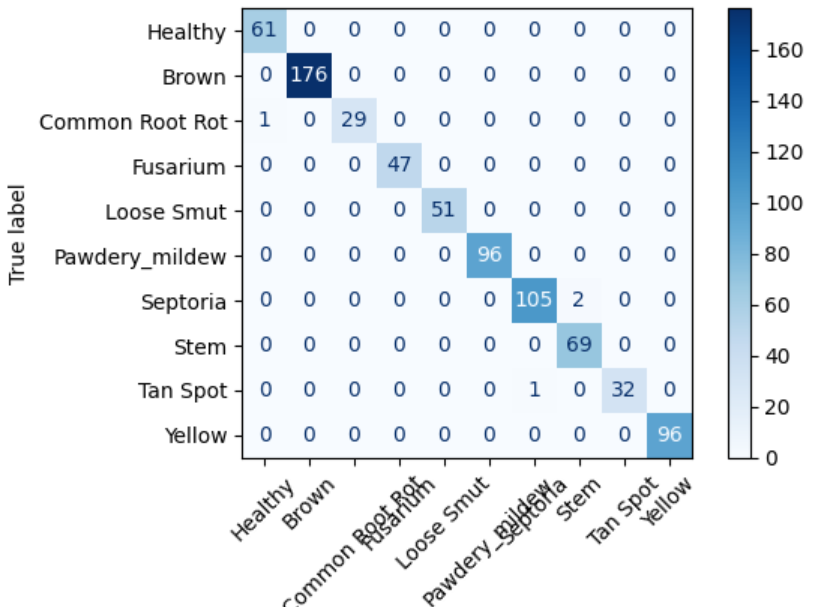
\includegraphics[width=0.8\textwidth]{chapters/chapter6/images/Figure04.png}
\caption{Confusion Matrix of the Hierarchical Classification System.}
\label{fig:confusion_hierarchical}
\end{figure}





\section{Comparison with the State of the Art}

In this section, we justify the choice of our hierarchical classification approach, which employs two models: a binary classifier followed by a multiclass classifier. This design decision was made to improve the overall accuracy and robustness of the classification pipeline, particularly for minimizing false alarms when detecting healthy plants.

Instead of using a single monolithic model to classify all categories, we propose first detecting whether a plant is healthy or not using a highly accurate binary classifier. If the sample is identified as unhealthy, a second multiclass classifier is then used to determine the specific disease. This separation allows the first model to specialize in identifying healthy vs. diseased plants with extreme accuracy, and the second model to focus on the subtler task of disease classification. This leads to enhanced performance and better generalization.

Our first model achieved an accuracy exceeding 99.66\%, efficiently fulfilling one of the key goals of this research: minimizing false alarms when identifying healthy plants. The second model, dedicated to disease classification, reached an accuracy of 99.86\%, further confirming the effectiveness of this hierarchical strategy.

To evaluate our approach, we compare it with the methodologies proposed in two recent state-of-the-art studies. The implementation of all approaches, including ours, was carried out under the same development environment and using our constructed dataset (due to unavailability of the original datasets used in those studies). The selection of these papers was based on several criteria, including the reproducibility of hyperparameters, availability of implementation details, and relevance to real-world applications. Results are presented in Table~\ref{tab:comparison_state_of_art}

\begin{itemize}
    \item \textbf{A Deep Learning Approach for Automated Wheat Disease Classification \parencite{oyal2021leaf}}: This method utilizes a deep CNN composed of 24 layers, trained on leaf and spike images. The architecture features multiple convolutional blocks with increasing filter sizes (64, 128, 256, 512) and dropout layers (0.25 after convolution and 0.5 in dense layers) to mitigate overfitting. Data augmentation is used during training, and the model is optimized using the Adam optimizer. It achieved a test accuracy of 92.74\% with an average inference time of 1.13 ms per image.

    \item \textbf{Lightweight Multiscale CNN Model for Wheat Disease Detection \parencite{fang2023lightweight}}: The proposed IRCE model combines Inception blocks with residual modules and integrates CBAM and ECA attention mechanisms. It aims to reduce complexity for mobile applications while preserving high accuracy. It achieved an accuracy of 85\% with an average inference time of 1.26 ms per image.
\end{itemize}    

\begin{table}[H]
\centering
\renewcommand{\arraystretch}{1.3}
\setlength{\tabcolsep}{6pt}
\caption{Comparative results between our Approach and two State-of-the-Art methods}
\begin{tabular}{|p{3cm}|p{2cm}|p{2cm}|p{2cm}|p{2cm}|p{2.5cm}|}
\hline
\textbf{Approach} & \textbf{Accuracy (\%)} & \textbf{Precision (\%)} & \textbf{Recall (\%)} & \textbf{F1-score (\%)} & \textbf{Avg Inference Time (ms)} \\
\hline
Deep CNN (24 layers) & 92.74 & 93.77 & 91.80 & 92.54 & 1.13 \\
\hline
IRCE Model & 85.00 & 83.00 & 82.00 & 82.00 & 1.26 \\
\hline
Ours (Hierarchical) & \textbf{99.48} & \textbf{99.38} & \textbf{99.18} & \textbf{99.31} & \textbf{1.08} \\
\hline
\end{tabular}
\label{tab:comparison_state_of_art}
\end{table}




Our hierarchical approach significantly outperforms the state-of-the-art models in all major evaluation metrics, including accuracy, precision, recall, and F1-score. The inference time is also competitive, making our solution not only accurate but also efficient. The two-step classification pipeline helps isolate healthy samples early, thereby reducing the computational load on the second classifier and minimizing false alarms. This targeted processing proves particularly beneficial in precision agriculture settings, where reducing misclassifications is crucial.

The detailed design and exceptional performance of both models validate the advantage of a hierarchical strategy over a single end-to-end model for this task.

\section{Evaluating Insect Pest Detection Model}

To evaluate the performance of our insect pest detection model, we created and annotated a dedicated dataset. The annotation process was conducted in two phases:

\begin{itemize}
    \item \textbf{First Phase – Standard Bounding Boxes (YOLOv8)}: In the initial phase, we used regular (horizontal) bounding boxes aligned with image axes. Each insect instance was enclosed in a rectangular box defined by four parameters: $(x, y, w, h)$, representing the top-left coordinates and width/height of the box.
    
    \item \textbf{Second Phase – Oriented Bounding Boxes (YOLOv8-OBB)}: In the second phase, we used oriented bounding boxes (OBBs), which allow for rotation. These are defined by five parameters: $(x, y, w, h, \theta)$, where $\theta$ indicates the angle of rotation. This approach enables more precise localization, especially for insects captured at various orientations.
\end{itemize}

We trained and evaluated two versions of the YOLOv8 model on the same dataset using two different annotation styles: one with standard bounding boxes and the other with oriented bounding boxes. The evaluation results are summarized in Table~\ref{tab:yolo_comparison}, which clearly shows that the YOLOv8-OBB variant outperforms the standard version across all key metrics.
\begin{table}[H]
\centering
\renewcommand{\arraystretch}{1.5}
\setlength{\tabcolsep}{8pt}
\caption{Comparison Between YOLOv8 with Oriented Bounding Boxes (OBB) and Standard YOLOv8}
\begin{tabular}{|c|c|c|p{6cm}|}
\hline
\textbf{Metric} & \textbf{YOLOv8-OBB} & \textbf{YOLOv8 (Standard)} & \textbf{Interpretation} \\
\hline
Precision (P) & 0.945 & 0.809 & OBB predicts fewer false positives. \\
\hline
Recall (R) & 0.862 & 0.564 & OBB detects more true positives. \\
\hline
mAP@0.5 & 0.924 & 0.708 & OBB shows much higher detection quality at 0.5 IoU. \\
\hline
mAP@0.5:0.95 & 0.683 & 0.474 & OBB performs better across stricter IoU thresholds. \\
\hline
\end{tabular}
\label{tab:yolo_comparison}
\end{table}


The results demonstrate the superior performance of the oriented bounding box approach across all evaluation metrics(See figure ~\ref{fig:detecres} ). The OBB-based model achieved significantly higher precision and recall, indicating that it is better at correctly identifying insect pests with fewer false detections. The mAP@0.5 and mAP@0.5:0.95 values confirm that the OBB model maintains higher accuracy, even under stricter Intersection over Union (IoU) thresholds. This improved performance is attributed to the OBB’s ability to more tightly and accurately fit insects that appear in varied poses and orientations, making it more suitable for real-world field conditions.


\begin{figure}[H] % 'H' needs \usepackage{float}
    \centering
    
\includegraphics[width=0.95\textwidth]{chapters/chapter6/images/Figure05.png}
    \caption{Insect detection model results.}
    \label{fig:detecres}
\end{figure}



\section*{Conclusion}

In this chapter, we conducted an in-depth evaluation of our proposed models through a set of carefully designed experiments. We focused first on the hierarchical classification approach for wheat disease detection, where the task was divided into two stages: a binary classifier to distinguish healthy from diseased plants, followed by a multiclass classifier to identify specific diseases. This structure led to superior performance across all key evaluation metrics—accuracy, precision, recall, and F1-score—outperforming existing state-of-the-art approaches while maintaining an efficient inference time.

Additionally, we assessed our insect pest detection model using both standard and oriented bounding boxes. The results clearly showed that the YOLOv8-OBB variant provided better localization and higher detection performance across all metrics. These promising outcomes confirm the effectiveness of our design choices and demonstrate the potential of our system for real-world applications in precision agriculture, particularly in early disease diagnosis and pest monitoring.